\documentclass[12pt, twoside]{article}
% \documentclass[12pt, twoside]{article}
\usepackage[letterpaper, margin=1in, headsep=0.2in]{geometry}
\setlength{\headheight}{0.6in}
%\usepackage[english]{babel}
\usepackage[utf8]{inputenc}
\usepackage{microtype}
\usepackage{amsmath}
\usepackage{amssymb}
%\usepackage{amsfonts}
\usepackage[nomessages]{fp} %\FPeval{\var-name}{2*sin(pi/6)}
\usepackage{siunitx} %units in math. eg 20\milli\meter
\usepackage{yhmath} % for arcs, overparenth command
\usepackage{tikz} %graphics
\usetikzlibrary{quotes, angles, arrows, arrows.meta}
\usepackage{graphicx} %consider setting \graphicspath{{images/}}
\usepackage{parskip} %no paragraph indent
\usepackage{enumitem}
\usepackage{multicol}
\usepackage{venndiagram}

\usepackage{fancyhdr}
\pagestyle{fancy}
\fancyhf{}
\renewcommand{\headrulewidth}{0pt} % disable the underline of the header
\raggedbottom
\hfuzz=2mm %suppresses overfull box warnings

\usepackage{hyperref}

\fancyhead[LE]{\thepage}
\fancyhead[RO]{\thepage \\ Name: \hspace{4cm} \,\\}
\fancyhead[LO]{BECA / Dr. Huson / Geometry\\*  Unit 8: Regents review\\* 28 May 2025}

\begin{document}

\subsubsection*{8.6 Classwork: Parallel \& perpendicular slopes, applications \hfill HSG.GPE.B.5}
\begin{enumerate}[itemsep=2cm]
\item What is the slope of a line parallel to the line with the equation $y=2x+5$?

\item What is an equation of the line that passes through the point $(6,8)$ and is parallel to a line with equation $y=\frac{3}{2}x+5$?
  \begin{multicols}{2}
    \begin{enumerate}
      \item $y-8=\frac{3}{2}(x-6)$
      \item $y-8=-\frac{3}{2}(x-6)$ 
      \item $y+8=\frac{3}{2}(x+6)$
      \item $y+8=-\frac{3}{2}(x+6)$
    \end{enumerate}
  \end{multicols}

\item What is an equation of the image of the line $\displaystyle y=\frac{3}{2}x-4$ after a translation up 3?

\item What equation represents a line with a $y$-intercept of $b=3$ that is perpendicular to the line represented by $\displaystyle y=\frac{2}{3}x+1$?
    
\item Determine and state an equation of the line perpendicular to the line\\ $5x-4y=10$ and passing through the point $(5,12)$. \vspace{1cm}

\item Write an equation of the line that is parallel to the line whose equation is $3y+7=2x$ and passes through the point $(2,6)$. \vspace{1cm}

\newpage
\item A translation maps $\overline{MN} \rightarrow \overline{M'N'}$. If $\overline{MN}$ is represented by $y=-3x+6$, which equation can represent $\overline{M'N'}$, the image of $\overline{MN}$?
  \begin{multicols}{2}
    \begin{enumerate}
      \item $y=-3x+12$
      \item $y=\frac{1}{3}x+6$ 
      \item $y=3x+12$
      \item $y=-\frac{1}{3}x+6$
    \end{enumerate}
  \end{multicols}

\item Show that quadrilateral $ABCD$ is a parallelogram. $A(0,3)$, $B(6,5)$, $C(8,2)$, $D(2,0)$
\begin{flushright}
  \begin{tikzpicture}[scale=0.6]
    \draw[help lines] (-2,-2) grid (8,8);
    \draw[thick, ->] (-2,0) -- (8.4,0) node [below right] {$x$};
    \draw[thick, <->] (0,-2.4)--(0,8.4) node [left] {$y$};
    \draw[thick] (0,3)node[left]{$A$}--
      (6,5)node[above]{$B$}--
      (8,2)node[right]{$C$}--
      (2,0)node[below]{$D$}--cycle;
  \end{tikzpicture}
\end{flushright}

\item Show that triangle $ABC$ is a right triangle. $A(0,3)$, $B(10,8)$, $C(4,0)$
\begin{flushright}
  \begin{tikzpicture}[scale=0.6]
    \draw[help lines] (-2,-2) grid (10,8);
    \draw[thick, ->] (-2,0) -- (10.4,0) node [below right] {$x$};
    \draw[thick, <->] (0,-2.4)--(0,8.4) node [left] {$y$};
    \draw[thick] (0,3)node[left]{$A$}--
      (10,8)node[above]{$B$}--
      (4,0)node[below]{$C$}--cycle;
  \end{tikzpicture}
\end{flushright}


\end{enumerate}
\end{document}